\documentclass[12pt, letterpaper]{article}
\usepackage{graphicx}

\title{Marine Heat waves}
\author{James Munroe}
\date{August 2, 2020}

\begin{document}

\maketitle

\section{Introduction}

In September 2019, a high temperature event in Fortune Bay resulted in the die-off salmon at an aquaculture site in Fortune Bay. The media reported this as significant event for the Newfoundland and Labrador \footnote{https://www.cbc.ca/news/canada/newfoundland-labrador/fortune-bay-cleanup-1.5305994} and the event and its clean up was the subject of public discussion. 
 
The ocean temperature near the surface (known as the sea surface temperature or SST) under goes daily and monthly variability superimposed on both a daily and annual cycle.  It important to understand how common a high temperature events are the ocean, how long they could last, and how significant the temperature anomaly is from the seasonal norms for a particular area.  While the specifics of the September 2019 die-off are not investigated here, we look at some ocean temperatures the same geographic region and describe the frequency and severity of abnormally warm periods.

\section{Methods}

\subsection{Dataset}

There are many ways to measure SST include from instruments deployed from boat, remote observations from satellites, and moored buoys.  In this report we will look at marine buoys are part of the Environment Canada Meteorological Service of Canada (MSC) buoy network.  This data is available for download from http://www.meds-sdmm.dfo-mpo.gc.ca/isdm-gdsi/waves-vagues/data-donnees/index-eng.asp as CSV files. The format of the CSV files is documented here http://www.meds-sdmm.dfo-mpo.gc.ca/isdm-gdsi/waves-vagues/formats-eng.html. In particular, depending on the model of the marine buoy, several data field are available as shown in Table~\ref{tbl:datafields}. Measuring sea surface temperature is not straightforward since there are many definition of precisely where the temperature is being measured.  For this report, we will focus on \texttt{SSTP} as the variable of interest.

\begin{table}[h]
\begin{tabular}{|l|l|}
\hline
Variable & Description and units                                                      \\ \hline
\texttt{WDIR }    & Direction from which the wind is blowing ($^\circ$ True)                          \\
\texttt{WSPD}     & Horizontal wind speed (m/s)                                                \\
\texttt{WSS\$}    & Horizontal scalar wind speed (m/s)                                         \\
\texttt{GSPD}    & Gust wind speed (m/s)                                                      \\
\texttt{ATMS}     & Atmospheric pressure at sea level (mbar)                                   \\
\texttt{DRYT}     & Dry bulb temperature ($^\circ$ C)                                                  \\
\texttt{SSTP}     & Sea surface temperature ($^\circ$ C)                                               \\
\texttt{SLEV}     & Observed sea level                                                         \\
\texttt{SST1}     & Average sea temperature from the non-synoptic part \\
  & of WRIPS buoy data ($^\circ$ C) \\
\texttt{HAT\$}    & Water temperature from high accuracy \\ & temperature sensor ($^\circ$ C)               \\ \hline
\end{tabular}
\caption{Variables in marine buoy data}
\label{tbl:datafields}
\end{table}

Specifically we look at the data from Station 44255 - NE Burgeo Bank. This marine buoy is owned and maintained by Environment and Climate Change Canada. It is 6-meter NOMAD buoy located at 47.270 N 57.340 W.  There is data available for this buoy from 1998 until 2017.  

\subsection{Marine Heat Waves}

To quantify whether SST for a particular area is indeed abnormally warm, we will use the Marine Heatwave (MHW) definition of Hobday et al. (manuscript submitted to Progress in Oceanography).  An algorithm for detecting a MHW has been implemented in the Python package `marineHeatWave`.

\section{Results}

As shown in Figure~\ref{fig:sst_timeseries}, the SST has a typical annual cycle between about $0^\circ$ C and $20^\circ$ C. There is some missing data between the years 2002 and 2004.  In 2005, 2006, and 2008 there is
increased noise in the data suggesting that something is wrong with the data.  It would be strange for the SST to be considerably below zero.  More significantly, the data from early 2010 is very suspicious as it suggests that the temperature is getting close to $80^\circ$ C.  Clearly we need to clean this dataset before continuing to analyze it.

\begin{figure}
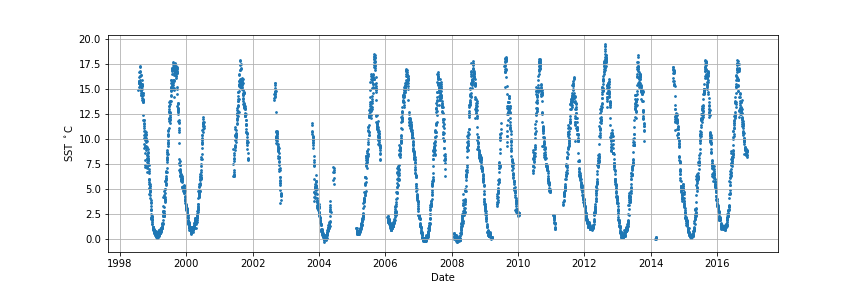
\includegraphics[width=0.9\textwidth]{sst_timeseries}
\caption{SST over time from at Station 44225}
\label{fig:sst_timeseries}
\end{figure}

This dataset from the Marine Environmental Data Section (MEDS) of the Department of Fisheries and Oceans (DFO) has already gone a quality control (QC) process. The results of QC are given by a numerical code as describe in Table~\ref{tbl:qc_codes}.

\begin{table}[h]
\begin{tabular}{|l|l|l|}
\hline
Code & Label & Description \\
\hline
0 & Blank & No quality control (QC) has been performed \\
1 & Good & QC has been performed: record appears correct \\
3 & Doubtful &  QC has been performed: record appears doubtful \\
4 & Erroneous & QC has been performed: record appears erroneous \\
5 & Changes & The record has been changed as a result of QC \\
6 & Acceptable & QC has been performed: record seems \\  & & inconsistent with other records \\
7 & Off Position & There is a problem with the buoy position or \\ & & mooring. Data may still be useful. \\
\hline
\end{tabular}
\caption{Quality control flags used in the marine buoy dataset}
\label{tbl:qc_codes}
\end{table}

\begin{figure}
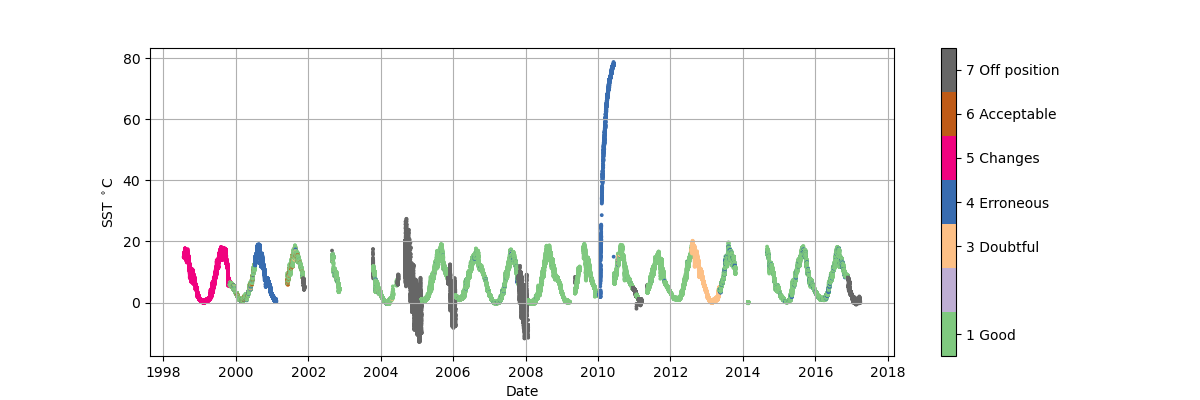
\includegraphics[width=0.9\textwidth]{qc_sst_timeseries}
\caption{SST over time from at Station 44225 with QC codes shown}
\label{fig:qc_sst_timeseries}
\end{figure}

\begin{figure}
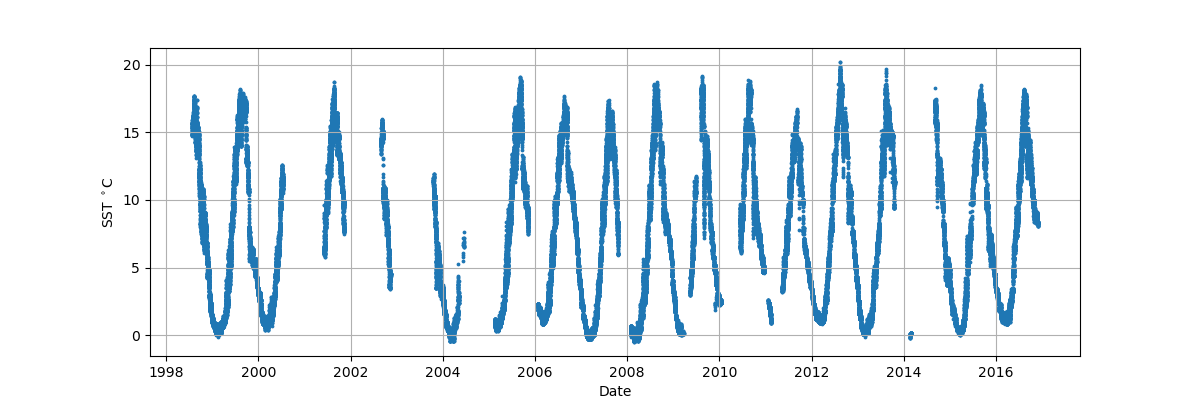
\includegraphics[width=0.9\textwidth]{filtered_sst_timeseries}
\caption{SST over time from at Station 44225 with only QC codes of 1, 3, 5, or 6 shown}
\label{fig:filterd_sst_timeseries}
\end{figure}

\begin{figure}
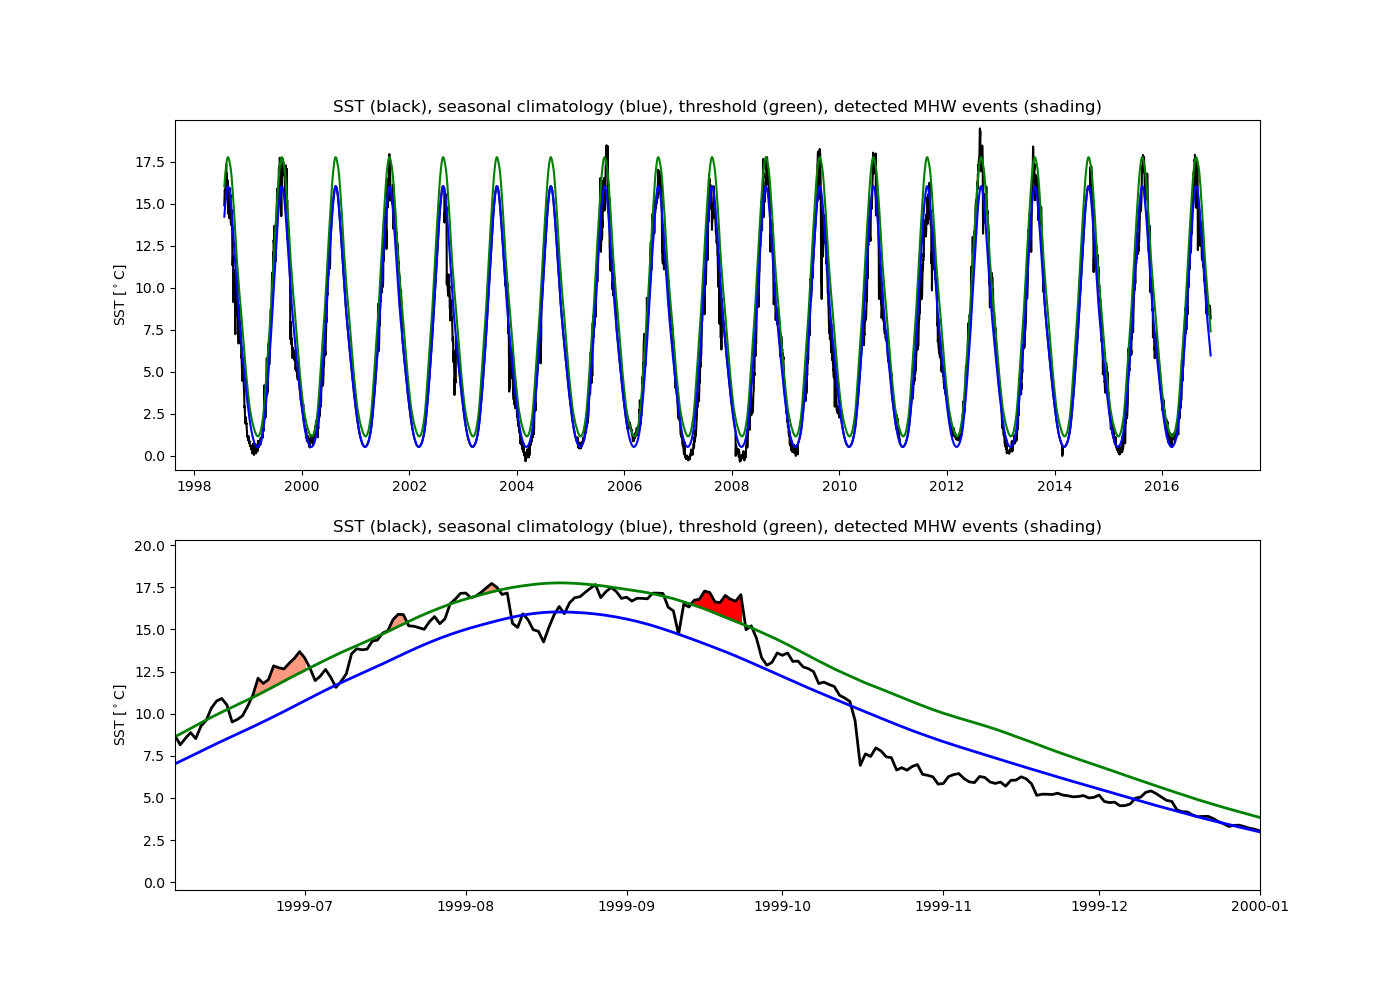
\includegraphics[width=0.9\textwidth]{mhw_timeseries}
\caption{marine heat waves}
\label{fig:mhw_timeseries}
\end{figure}

\begin{figure}
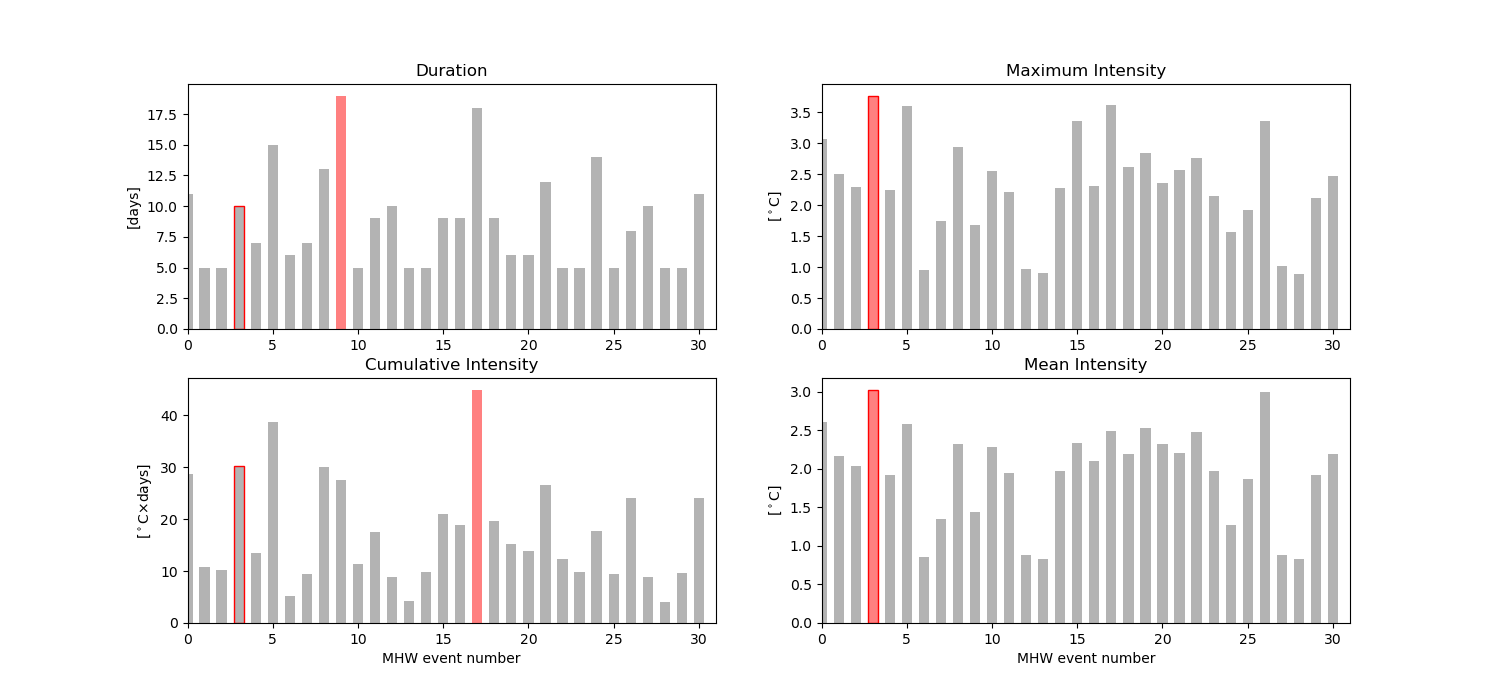
\includegraphics[width=0.9\textwidth]{mhw_distribution}
\caption{Distribution of marine heat waves over time}
\label{fig:distribution}
\end{figure}



\section{Conclusions}


% would be good to a a bibiography here too.

\end{document}
